% \newpage
% \section{ДЕТАЛІ ВПРОВАДЖЕННЯ}
% У розділі наведено інформацію про деталі реалізації експериментів, ціллю яких є знаходження оптимальних параметрів розглянутих алгоритмів рекомендацій на основі результатів метрик якості. А також порівняння впливу не залежних від моделі факторів.

% \subsection{Датасети}
% \begin{figure}[H]
%     \centering
%     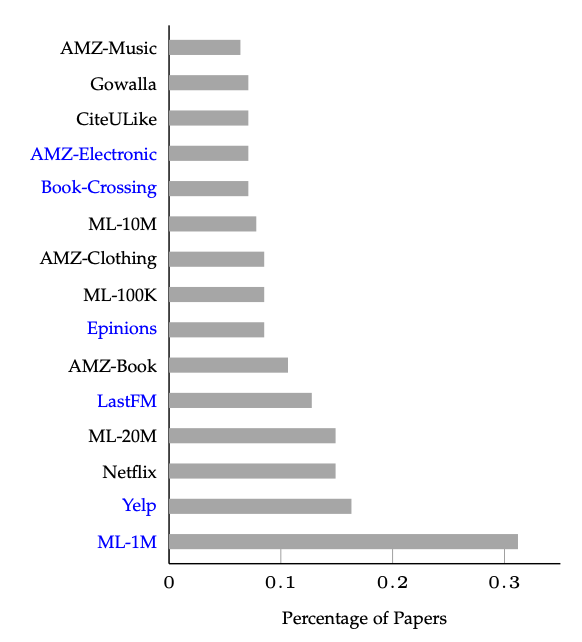
\includegraphics[width=0.6\textwidth]{images/dataset_dist.png}
%     \caption{Розподіл використання наборів даних у наукових статтях.}
% \end{figure}
% Для практичних еспериментів, а також навчання і валідації моделей будо обрано відкриті набори даних які є загально прийняті і використовуються для порівняння у академічній сфері (Рис. 18). Для кожного датасету проведений розвідувальний аналіз даних (EDA) для оприділення їх основних структурних особливостей і відмінностей. Кожен набір є зрізом БД приватних комерційних компаній, тому можна вважати що поведінка моделей відповідає реальним результатам.

% \subsubsection{Movielens 1M \cite{MovilensDataset}}
% Набір даних Movielens (ML-1M) є найпопулярнішим серед великого різноманіття датасетів. Movielens -  це мережева система рекомендацій фільмів для користувачів на базі їх відгуків і оцінок. Існує із 1996 року і містить у собі більше 11 мільйонів оцінок для 8600 об’єктів.
% \begin{figure}[H]
%     \centering
%     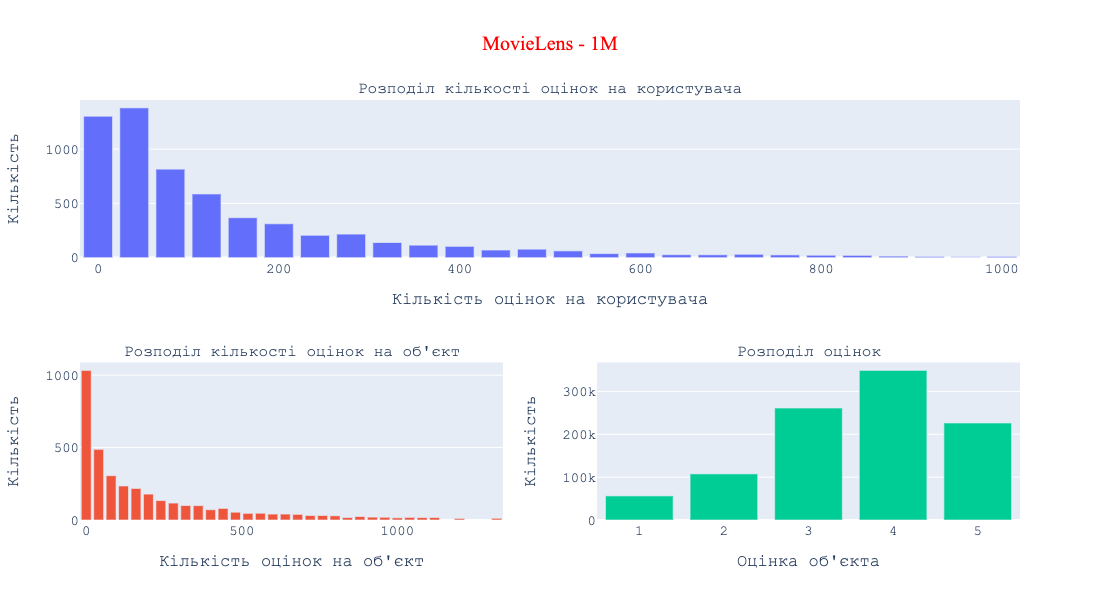
\includegraphics[width = 1\textwidth]{images/ML-1m_stat.png}    
%     \caption{EDA для набору даних Movielens (ML-1M) }
% \end{figure}
% Структура набору наступна: 
% \begin{itemize}
%     \item $item\_id$ індентифікатор користувача.
%     \item $user\_id$ індентифікатор об’єкта рекомендацій.
%     \item $score$ оцінка.
%     \item $timestamp$ дата і час дії.
% \end{itemize}

% Для аналізу відібрано 3706 об’єктів рекомендацій (фільмів) із 1 000 036  оцінок від корисутувачів. Що надає не менше 20 відгуків на один об’єкт.
% \begin{table}[H]
%     \centering
%     \caption{Характеристика набору даних Movielens 1M}
%     \begin{tabular}{|c|c|}
%         \hline
%         Загальна статистика      & Значення \\ \hline
%         Кількість взаємодій      & 1 000 029                    \\
%         Кількість користувачів   & 6 040                        \\
%         Кількість об’єктів       & 3 706                        \\
%         Розрідженність           & 99.9553\%                    \\
%         Середня оцінка           & 3.58 / 5                     \\ \hline
%         Взаємодій на користувача &                              \\ \hline
%         Середнє                  & 165.6                        \\
%         Медіана                  & 96.0                         \\ \hline
%         Взаємодій на об’єкт      &                              \\ \hline
%         Середнє                  & 269.89                       \\
%         Медіана                  & 123.5                        \\ \hline
%     \end{tabular}
%     \label{tab:ML-1m}
% \end{table}
% Більшість оцінок приймають значення від 3 до 4-5. У розподілі взаємодій чітко замітний лівий перекіс, що типово для даних такого роду. Розрідженість висока.


% \subsubsection{LastFm \cite{LastFMDataset}}
% Набір даних LastFm містить у собі інформацію про музику яка прослуховується у медіа плеєрах користувачів. Структурно датасет подібний до ML-1M, але додатково присутня інформація про ключові теги класу для об’єктів. Теги можуть описувати жанр, автора, додаткову ключову інформацію, що є зручним і може бути використано для насичення моделей.


% \begin{figure}[H]
%     \centering
%     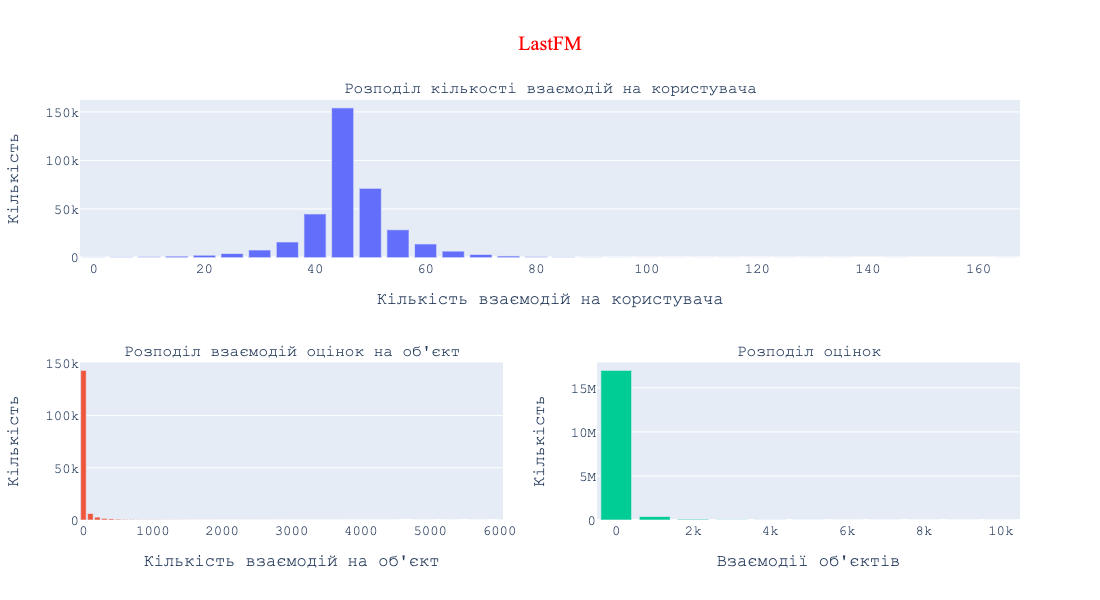
\includegraphics[width = 1\textwidth]{images/LastFM_stat.png}    
%     \caption{EDA для набору даних Last.fm}
% \end{figure}

% \begin{table}[H]
%     \centering
%     \caption{Характеристика набору даних LastFM}
%     \begin{tabular}{|c|c|}
%         \hline
%         Загальна статистика      & Значення \\ \hline
%         Кількість взаємодій      & 17 535 654                    \\
%         Кількість користувачів   & 358 868                        \\
%         Кількість об’єктів       & 160 113                        \\
%         Розрідженність           & 99.9996\%                    \\\hline
%         Взаємодій на користувача &                              \\ \hline
%         Середнє                  & 48.23                        \\
%         Медіана                  & 48.0                         \\ \hline
%         Взаємодій на об’єкт      &                              \\ \hline
%         Середнє                  & 108.10                       \\
%         Медіана                  & 6.0                        \\ \hline
%     \end{tabular}

%     \label{tab:LastFM}
% \end{table}

% \subsubsection{Netflix \cite{NetflixDataset}}
% Набір даних Netflix є одним із найбільших відкритих датасетів із реальними даними. Набір був створений під егідою проведення змагання Netflix Prize. Ціллю якого було розробка системи рекомендацій, переможець який добився найвищих показників якості отримав призову винагороду у розмірі 1 мільйон доларів. Датасет має класичну структуру: включає у собі дані про оцінки користувачів фільмів які були переглянути користувачами. Для кожного екземпляру є відмітка про час оцінки. 

% Дані мають типовий розподіл, і явно замітний перекіс. Із цікавого, через великий розмір і характер домену (рекомендація фільмів), датасет є одним із найнасичених. Розподіл оцінок - стандартний ([3, 4, 5]). Більше 90\% користувачів оцінили менше ста об’єктів.
% \begin{figure}[H]
%     \centering
%     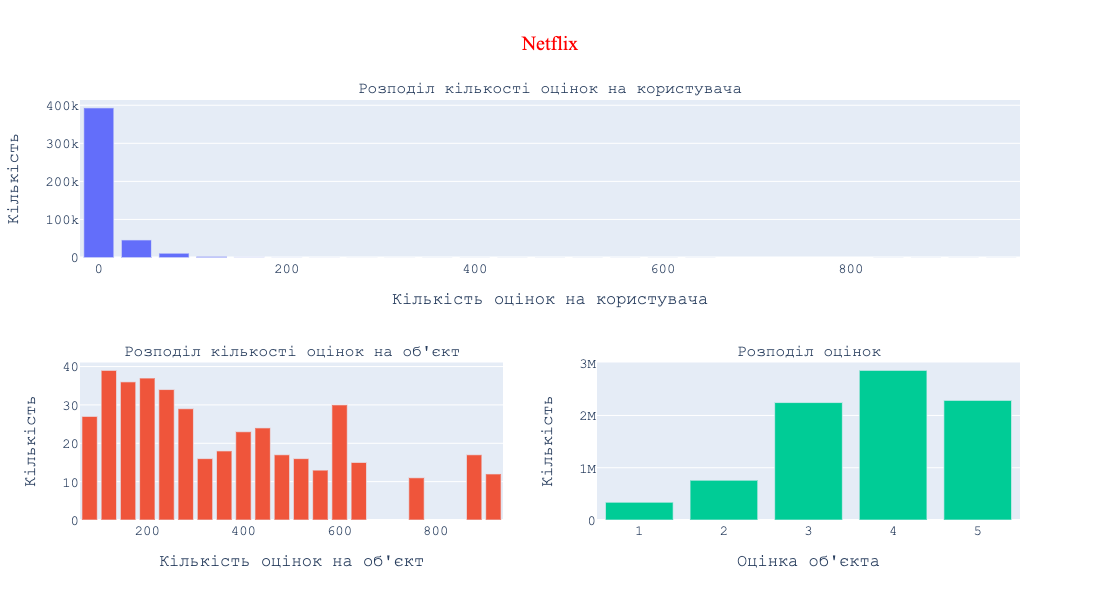
\includegraphics[width = 1\textwidth]{images/netflix_stat.png}    
%     \caption{EDA для набору даних Netflix}
% \end{figure}
% У Таблиці 7.3 наведено докладна характеристика набору.
% \begin{table}[H]
%     \centering
%     \caption{Характеристика набору даних Netflix}
%     \begin{tabular}{|c|c|}
%         \hline
%         Загальна статистика      & Значення \\ \hline
%         Кількість взаємодій      & 100 480 507                  \\
%         Кількість користувачів   & 480 189                        \\
%         Кількість об’єктів       & 17 770                        \\
%         Розрідженність           & 98.8239\%                    \\\hline
%         Взаємодій на користувача &                              \\ \hline
%         Середнє                  & 209.33                       \\
%         Медіана                  & 87.0                         \\ \hline
%         Взаємодій на об’єкт      &                              \\ \hline
%         Середнє                  & 5654.50                       \\
%         Медіана                  & 967                      \\ \hline
%     \end{tabular}
%     \label{tab:Netflix}
% \end{table}

% Середня кількісь оцінок на об’єкт є надзвичайно високою.
% \subsection{Середовище розгортання}

% Експермиментальне дослідження проводиться на базі сервісу хмарних обчислень  Google Colab. Для навчання використано GPU Nvidia Tesla K80. Дані датасетів отримані із офіційних сторінок, розміщені у хмарному сховищі у вигляді текстових документів. Версія Python 3.8.15. Моделі імплементовані із використпанням бібліотеки torch. 
% \subsection*{Висновки}
% Проведений аналіз наборів даних для побудови рекомендацій. Оцінено їх насиченість, частоту взаємодій відносно користувача і об’єкту. Наведено справочну інформацію про розмір, об’єм і структуру наборів. Вказано платформу реалізації практичних експериментів.